\chapter{Implémentation}
\label{chaper-2}

%Description fonctionnalités programme

%Explications implémentation de l'algorithme de ray-tracing, et de la structure du code


\section{Interface utilisateur}
Une interface graphique (visible Figure [\ref{fig:interface}]) a été créée afin de faciliter l'exécution de la simulation pour un utilisateur selon ses paramètres choisis, sans devoir recompiler le programme, ni entrer ces paramètres via une ligne de commande.\\

L'utilisateur peut choisir les coordonnées de la station de base ainsi que le mode de simulation:
\begin{itemize}
    \item Une \textit{heatmap} de la couverture,
    \item Des tracés de rayons jusqu'à une seule cellule réceptrice.
\end{itemize}

Le mode \textit{Coverage Heatmap} permet d'avoir le rendu de la couverture de l'appartement, où l'utilisateur peut choisir la résolution des cellules de la carte (leur largeur, allant de 0,5m à 0,0625m).

Quant au mode \textit{Rays to Single Cell}, il permet de visualiser tous les rayons simulés vers une unique cellule (de largeur 0,5m), où l'utilisateur peut choisir les coordonnées de cette cellule.\\

Des boutons grisés sont présents dans l'interface, ceux-ci représentent des fonctionnalités futures qui n'ont pas été encore implémentées par manque de temps pour ce projet.\\

Le haut de l'interface contient un large bouton \textit{Run simulation} qui permet de lancer la simulation avec les paramètres rentrés. Au-dessus de ce bouton se trouve un cadre qui affichera si la simulation s'est finie avec succès, ainsi que son temps d'exécution en millisecondes. En dessous du bouton se trouve une barre de progression de la simulation. Ceci est visible Figure [\ref{fig:time-0.125m}].\\

En haut de la fenêtre se trouve trois menus:
\begin{itemize}
    \item Le premier (\textit{Menu}) permet de sauvegarder une image de la simulation après son exécution, et permet également de réinitialiser l'application ou de la fermer.
    \item Le second (\textit{Info}) permet d'avoir des informations sur l'application, et donne aussi un lien vers le Github du projet.
    \item Le troisième (\textit{TP4-Simulation}) permet de lancer le rendu de la simulation de l'exercice 1 du TP4, ainsi que de sauvegarder une image de celui-ci.
\end{itemize}

\begin{figure}[H]
    \centering
    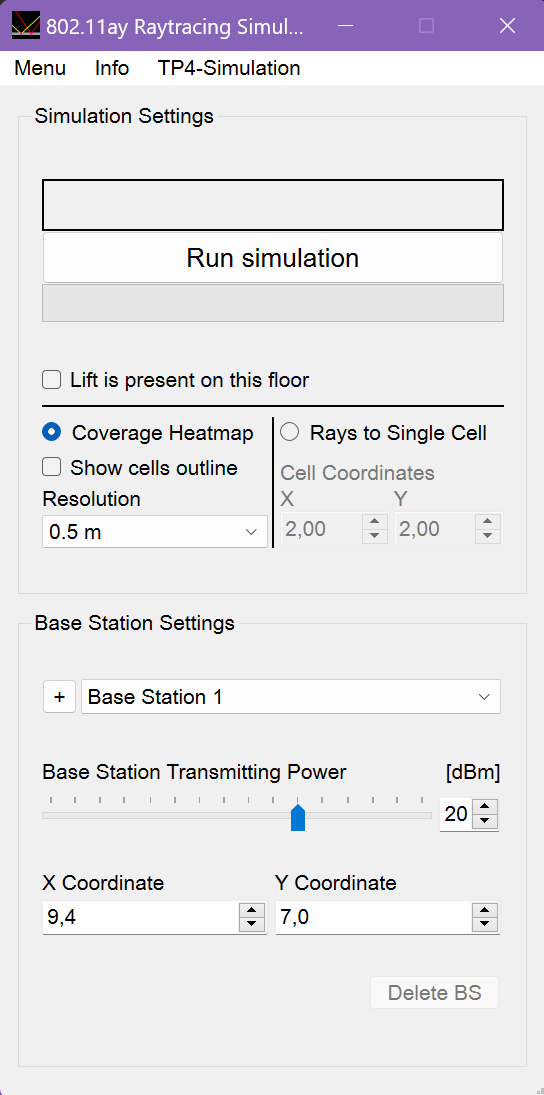
\includegraphics[width=0.5\textwidth]{latex/images/interface.png}
    \caption{Interface utilisateur du programme}
    \label{fig:interface}
\end{figure}

\section{Algorithme}
% TODO: explication algo
...

\section{Affichage}
Après l'exécution d'une simulation, l'application affiche à l'utilisateur une visualisation graphique de cette simulation. Un exemple vide est visible Figure [\ref{fig:blank-map}]. Elle présente une carte de l'appartement, les axes, ainsi qu'une légende. Les murs/parois sont représentés par des traits de couleurs et épaisseurs différentes représentant leurs matériaux. L'émetteur est représenté par un point blanc. Les cellules réceptrices seront représentées par des carrés de couleurs représentant leurs débits binaires selon le dégradé affiché dans la légende.
% TODO:

\begin{figure}[H]
    \centering
    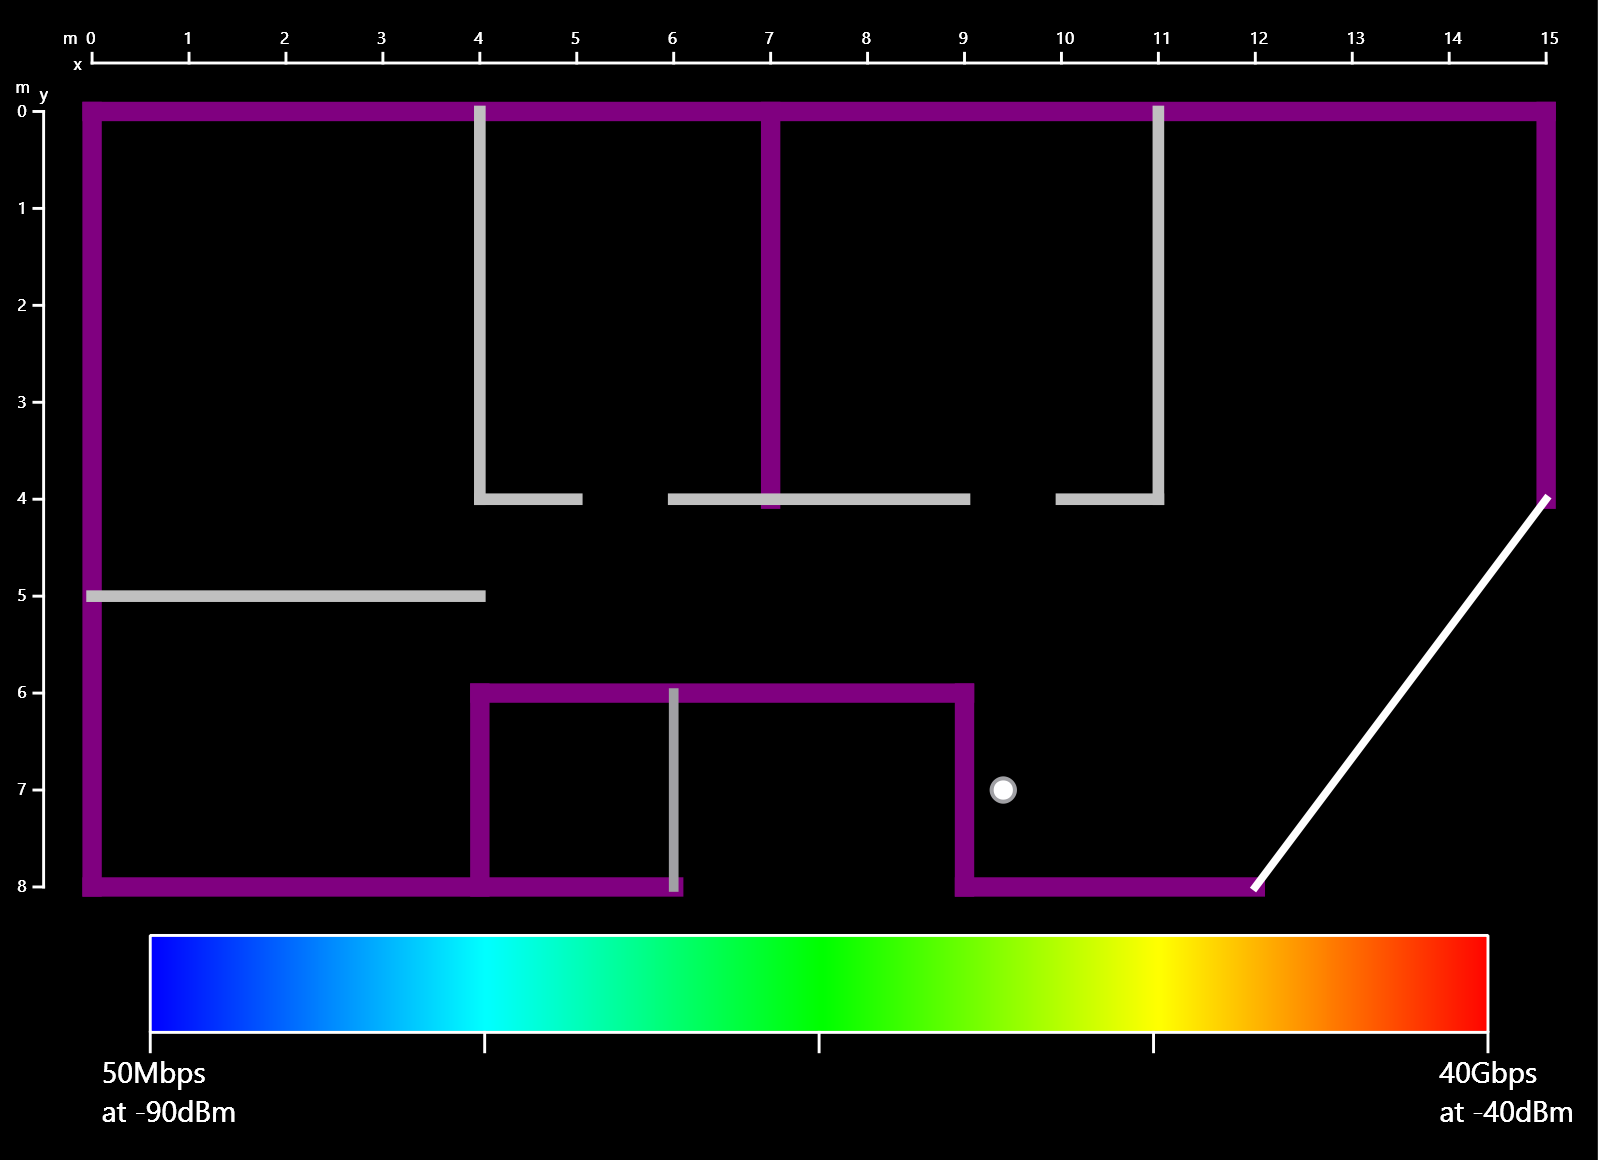
\includegraphics[width=\textwidth]{latex/images/blank_map.png}
    \caption{Carte vide de la simulation}
    \label{fig:blank-map}
\end{figure}

\section{Ajouts futurs possibles}
% décrire les futures ameliorations qui peuvent être ajoutées
Les ajouts et améliorations futurs possibles sont:
\begin{itemize}
    \item Simulation contenant plusieurs stations de base (comme visible grisé dans l'interface [Figure \ref{fig:interface}])
    \item Sélection du nombre maximal de réflexions des rayons (nécessitant un algorithme de ray-tracing récursif)
    \item Importation de différentes cartes d'appartement
    \item Mode d'optimisation de placement de station de base (par méthode de Monte-Carlo ou algorithme génétique)
\end{itemize}

\section{Performances}
% temps d'exécution, RAM etc
Le temps d'exécution pour une simulation exemple, de résolution de cellule de $0.125\mathrm{m}\times0.125\mathrm{m}$ est aux alentours des 500ms [Figure \ref{fig:time-0.125m}], avec une utilisation de 2,8GB de RAM, soit des performances tout à fait acceptables.

Le temps d'exécution a été calculé grâce à un objet \mintinline{cpp}{QTimer}, lancé après une pression du bouton \textit{Run simulation} et stoppé juste avant l'affichage graphique.
\begin{figure}[H]
    \centering
    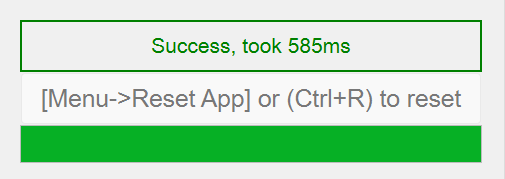
\includegraphics[width=0.7\textwidth]{latex/images/time-0.125m.png}
    \caption{Temps d'exécution simulation de résolution 0.125m}
    \label{fig:time-0.125m}
\end{figure}

Le temps d'exécution pour une simulation \textit{Rays to Single Cell}, ou pour la simulation du TP4, tourne autour des 2ms.
